\documentclass[a4paper]{article}

%% Language and font encodings
\usepackage[english]{babel}
\usepackage[utf8x]{inputenc}
\usepackage[T1]{fontenc}

%% Sets page size and margins
\usepackage[a4paper,top=3cm,bottom=2cm,left=3cm,right=3cm,marginparwidth=1.75cm]{geometry}

%% Useful packages
\usepackage{amsmath}
\usepackage{graphicx}
\usepackage[colorinlistoftodos]{todonotes}
\usepackage[colorlinks=true, allcolors=blue]{hyperref}
\usepackage{listings}
\usepackage{pgfplots}
\pgfplotsset{compat=1.14}

\title{Blurry Image Recognition}
\author{Ian Beamer}

\begin{document}
\maketitle

\begin{abstract}
A neural network can be trained to read human handwriting when tested on handwriting with the same level of sharpness to the image. This experiment trained the MNIST data set against a testing set that went through several blurring phases, and compared them to the original results. Results varied greatly based on the arrangement of the code, from incredibly low accuracy, to almost always being correct.
\end{abstract}

\section{Introduction}

MNIST is a large data set of handwritten numbers, and is a popular example when teaching students the fundamentals of deep learning. Due to the small size of the images, it can be run on most common computers in a relatively small amount of time. While being a good teaching tool, it can be incredibly beneficial to experiment on the dataset to see just what a neural network is capable of. \cite{Goodfellow-et-al-2016}

If a network can be trained to understand a normal set of handwritten numbers, what would happen if those images came in with some sort of corruption, such as a blurry or fuzzy image due to a poor image quality? This set of experiments sought to determine if this was possible.

\section{Neural Net Setup}
The network is taken directly from TensorFlow's example \cite{tensorflowTutorial} . The average MNIST image is 784 pixels large (28x28), and is entirely grayscale, allowing for an initial shape of 1, compared to the RGB size of 3. We can use a convolutional network to learn what each image may be. The first layer maps an image to 32 feature maps, adds a small bias, and uses a RELU activation function. The next layer pools the original layer, downsampling by 2. The second layer maps the 32 feature maps to 64 maps, adds a bias, and runs through a RELU activation function. The second pooling layer downsamples by 2 again. After this, a fully connected layer is formed, with a feature map of 7x7x64, and is mapped to 1024 features in this step. \cite{tensorflowSource}

\subsection{Original Training Setup}
\begin{lstlisting}
  with tf.Session() as sess:
    sess.run(tf.global_variables_initializer())
    for i in range(20000):
      batch = mnist.train.next_batch(50)
      if i % 100 == 0:
        train_accuracy = accuracy.eval(feed_dict={
            x: batch[0], y_: batch[1], keep_prob: 1.0})
        print('step %d, training accuracy %g' % (i, train_accuracy))
      train_step.run(feed_dict={x: batch[0], y_: batch[1], keep_prob: 0.5})

    print('test accuracy %g' % accuracy.eval(feed_dict={
      x: mnist.test.images, y_: mnist.test.labels, keep_prob: 1.0}))
\end{lstlisting}

This set of code has consistently come out with a 99.2 percent accuracy, and is decently quick to run, taking about 4-5 minutes to run fully.
 

\subsection{Training with Sharp Images, Testing with Blurred Images}
The three networks that were experimented upon runs much slower, taking nearly 5 hours to completely run.
This trains the network to recognize the original, unblurred images. Several attempts were made to rectify this issue. Starting with training the network on unsharpened images, then testing them against Gaussian blurs in a number of ways.

\begin{lstlisting}
  //gaussian_filter from SciPy library
  with tf.Session() as sess:
    sess.run(tf.global_variables_initializer())
    for i in range(20000):
      batch = mnist.train.next_batch(50)
      if i % 100 == 0:
        train_accuracy = accuracy.eval(feed_dict={
            x: batch[0], y_: batch[1], keep_prob: 1.0})
        print('step %d, training accuracy %g' % (i, train_accuracy))
      train_step.run(feed_dict={x: batch[0], y_: batch[1], keep_prob: 0.5})

    for j in range(100):
      print('test accuracy on blur level ' + str(j) + ': %g' % accuracy.eval(feed_dict={
      x: gaussian_blur(mnist.test.images, j), y_: mnist.test.labels, keep_prob: 1.0}))
\end{lstlisting}

The results were poor, illustrating exponential decay in accuracy. With the possibility that this method was somehow breaking the program, a new method was created.

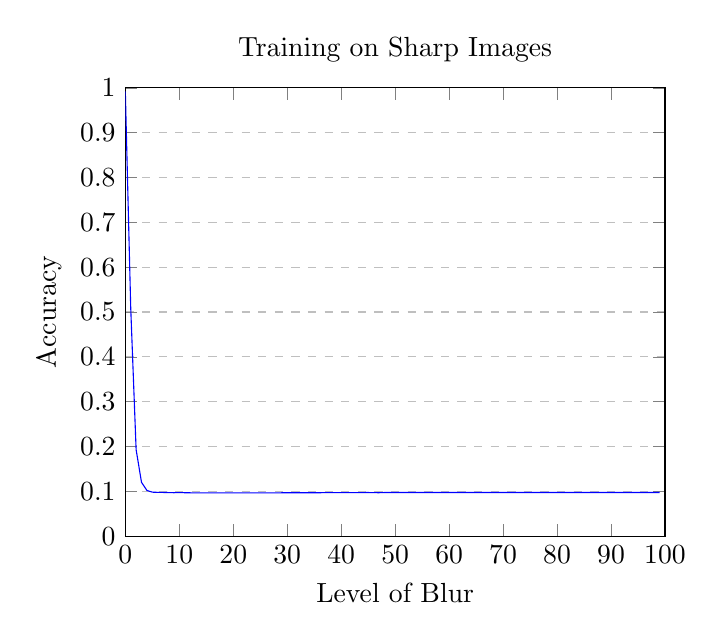
\begin{tikzpicture}
\begin{axis}[
    title={Training on Sharp Images},
    xlabel={Level of Blur},
    ylabel={Accuracy},
    xmin=0, xmax=100,
    ymin=0, ymax=1,
    xtick={0,10,20,30,40,50,60,70,80,90,100},
    ytick={0,0.1,0.2,0.3,0.4,0.5,0.6,0.7,0.8,0.9,1.0},
    ymajorgrids=true,
    grid style=dashed,
]
 
\addplot[
    color=blue,
    ]
    coordinates {
(0 , 0.992)
(1 , 0.5093)
(2 , 0.1929)
(3 , 0.1201)
(4 , 0.1021)
(5 , 0.0982)
(6 , 0.0978)
(7 , 0.0976)
(8 , 0.0973)
(9 , 0.097)
(10 , 0.0973)
(11 , 0.097)
(12 , 0.0968)
(13 , 0.0966)
(14 , 0.0967)
(15 , 0.0966)
(16 , 0.0966)
(17 , 0.0966)
(18 , 0.0966)
(19 , 0.0966)
(20 , 0.0966)
(21 , 0.0966)
(22 , 0.0966)
(23 , 0.0966)
(24 , 0.0966)
(25 , 0.0966)
(26 , 0.0967)
(27 , 0.0967)
(28 , 0.0967)
(29 , 0.0968)
(30 , 0.0968)
(31 , 0.0968)
(32 , 0.0969)
(33 , 0.0969)
(34 , 0.0969)
(35 , 0.097)
(36 , 0.097)
(37 , 0.0971)
(38 , 0.0971)
(39 , 0.0973)
(40 , 0.0973)
(41 , 0.0973)
(42 , 0.0973)
(43 , 0.0972)
(44 , 0.0973)
(45 , 0.0974)
(46 , 0.0971)
(47 , 0.097)
(48 , 0.0974)
(49 , 0.0974)
(50 , 0.0974)
(51 , 0.0974)
(52 , 0.0974)
(53 , 0.0974)
(54 , 0.0974)
(55 , 0.0974)
(56 , 0.0974)
(57 , 0.0974)
(58 , 0.0974)
(59 , 0.0974)
(60 , 0.0974)
(61 , 0.0974)
(62 , 0.0974)
(63 , 0.0974)
(64 , 0.0974)
(65 , 0.0974)
(66 , 0.0974)
(67 , 0.0974)
(68 , 0.0974)
(69 , 0.0974)
(70 , 0.0974)
(71 , 0.0974)
(72 , 0.0974)
(73 , 0.0974)
(74 , 0.0974)
(75 , 0.0974)
(76 , 0.0974)
(77 , 0.0974)
(78 , 0.0974)
(79 , 0.0974)
(80 , 0.0974)
(81 , 0.0974)
(82 , 0.0974)
(83 , 0.0974)
(84 , 0.0974)
(85 , 0.0974)
(86 , 0.0974)
(87 , 0.0974)
(88 , 0.0974)
(89 , 0.0974)
(90 , 0.0974)
(91 , 0.0974)
(92 , 0.0974)
(93 , 0.0974)
(94 , 0.0974)
(95 , 0.0974)
(96 , 0.0974)
(97 , 0.0974)
(98 , 0.0974)
(99 , 0.0974)
    };
 
\end{axis}
\end{tikzpicture}

\subsection{Training and Testing on Blurred Images}
\begin{lstlisting}
  with tf.Session() as sess:
    sess.run(tf.global_variables_initializer())
    for j in range(100):
      mnist = input_data.read_data_sets(FLAGS.data_dir, one_hot=True)
      for k in range(20000):  
        gaussian_filter(mnist.train.images[k], j)
      for i in range(20000):
        batch = mnist.train.next_batch(50)
        if i % 100 == 0:
          train_accuracy = accuracy.eval(feed_dict={
              x: batch[0], y_: batch[1], keep_prob: 1.0})
          print('step %d, training accuracy %g' % (i, train_accuracy))
        train_step.run(feed_dict={x: batch[0], y_: batch[1], keep_prob: 0.5})
      print('test accuracy on blur level ' + str(j) + ': %g' % accuracy.eval(feed_dict={
        x: gaussian_filter(mnist.test.images, j), y_: mnist.test.labels, keep_prob: 1.0}))
\end{lstlisting}

This setup experiences a slightly more gradual decay, but ultimately ends with about 10 percent accuracy, much like the previous setup. Notice how there is significantly more noise in the asymptotic region.

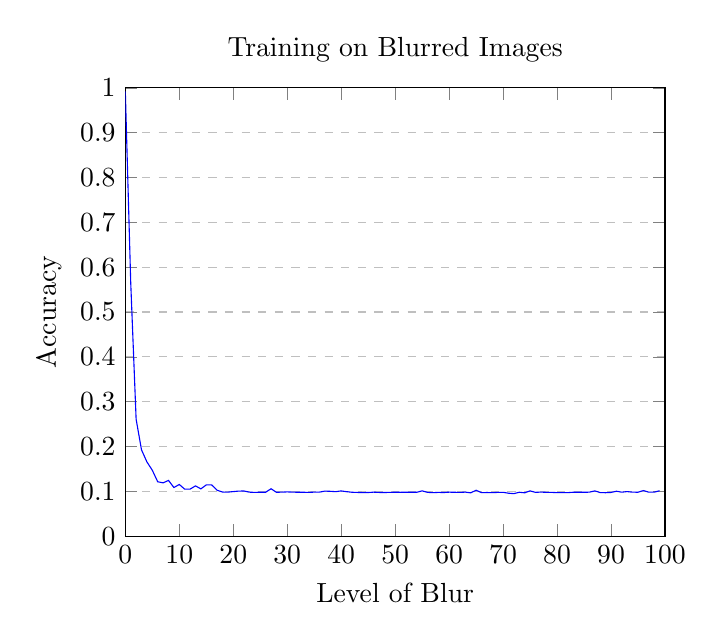
\begin{tikzpicture}
\begin{axis}[
    title={Training on Blurred Images},
    xlabel={Level of Blur},
    ylabel={Accuracy},
    xmin=0, xmax=100,
    ymin=0, ymax=1,
    xtick={0,10,20,30,40,50,60,70,80,90,100},
    ytick={0,0.1,0.2,0.3,0.4,0.5,0.6,0.7,0.8,0.9,1.0},
    ymajorgrids=true,
    grid style=dashed,
]
 
\addplot[
    color=blue,
    ]
    coordinates {
(0, 0.9921)
(1, 0.5659)
(2, 0.2609)
(3, 0.1925)
(4, 0.1657)
(5, 0.1471)
(6, 0.1214)
(7, 0.119)
(8, 0.1244)
(9, 0.1086)
(10, 0.1154)
(11, 0.1049)
(12, 0.105)
(13, 0.1122)
(14, 0.1056)
(15, 0.1144)
(16, 0.1144)
(17, 0.1026)
(18, 0.0985)
(19, 0.0983)
(20, 0.0995)
(21, 0.1006)
(22, 0.1008)
(23, 0.0982)
(24, 0.0977)
(25, 0.0981)
(26, 0.098)
(27, 0.1058)
(28, 0.0979)
(29, 0.0983)
(30, 0.0988)
(31, 0.0983)
(32, 0.098)
(33, 0.098)
(34, 0.0977)
(35, 0.0983)
(36, 0.0984)
(37, 0.1006)
(38, 0.1001)
(39, 0.0993)
(40, 0.101)
(41, 0.0993)
(42, 0.098)
(43, 0.0976)
(44, 0.0973)
(45, 0.0974)
(46, 0.0982)
(47, 0.0976)
(48, 0.0974)
(49, 0.0978)
(50, 0.098)
(51, 0.0979)
(52, 0.098)
(53, 0.098)
(54, 0.0979)
(55, 0.1011)
(56, 0.0978)
(57, 0.0971)
(58, 0.0977)
(59, 0.0974)
(60, 0.0982)
(61, 0.098)
(62, 0.0976)
(63, 0.0983)
(64, 0.0967)
(65, 0.1025)
(66, 0.0971)
(67, 0.0974)
(68, 0.0971)
(69, 0.0977)
(70, 0.0979)
(71, 0.0959)
(72, 0.0949)
(73, 0.098)
(74, 0.0968)
(75, 0.1011)
(76, 0.0978)
(77, 0.0984)
(78, 0.0978)
(79, 0.0977)
(80, 0.0972)
(81, 0.0973)
(82, 0.0972)
(83, 0.098)
(84, 0.098)
(85, 0.098)
(86, 0.0982)
(87, 0.1011)
(88, 0.0972)
(89, 0.097)
(90, 0.0976)
(91, 0.1003)
(92, 0.0982)
(93, 0.0995)
(94, 0.0982)
(95, 0.0981)
(96, 0.1018)
(97, 0.0982)
(98, 0.0982) 
(99, 0.1014)
    };
 
\end{axis}
\end{tikzpicture}

\subsection{Training and Testing on Blurred Images, Alternate Method}
\begin{lstlisting}
  with tf.Session() as sess:
    sess.run(tf.global_variables_initializer())
    for j in range(100):
      mnist = input_data.read_data_sets(FLAGS.data_dir, one_hot=True)
      for k in range(10000):
        gaussian_filter(mnist.test.images[k], j)
      for k in range(20000):  
        gaussian_filter(mnist.train.images[k], j)
      for i in range(20000):
        batch = mnist.train.next_batch(50)
        if i % 100 == 0:
          train_accuracy = accuracy.eval(feed_dict={
              x: batch[0], y_: batch[1], keep_prob: 1.0})
          print('step %d, training accuracy %g' % (i, train_accuracy))
        train_step.run(feed_dict={x: batch[0], y_: batch[1], keep_prob: 0.5})
      print('test accuracy on blur level ' + str(j) + ': %g' % accuracy.eval(feed_dict={
        x: mnist.test.images, y_: mnist.test.labels, keep_prob: 1.0}))
\end{lstlisting}


This setup seems to preform incredibly well, averaging at 99.4 percent accuracy.This could be a result of faulty methods, or possibly a really good setup. Note how the graph starts out at 0.992, and how it never passes 99.5 percent accuracy.

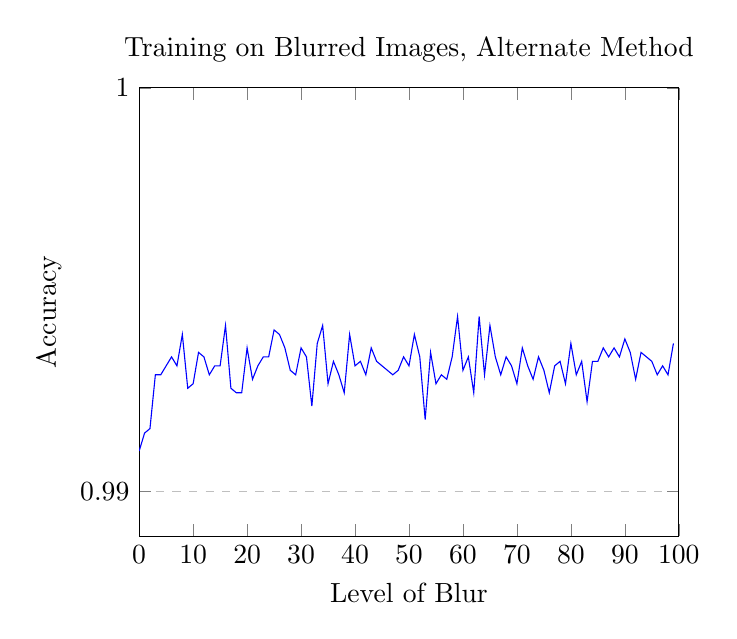
\begin{tikzpicture}
\begin{axis}[
    title={Training on Blurred Images, Alternate Method},
    xlabel={Level of Blur},
    ylabel={Accuracy},
    xmin=0, xmax=100,
    ymin=.99, ymax=1,
    xtick={0,10,20,30,40,50,60,70,80,90,100},
    ytick={0.90,0.991,1.0},
    ymajorgrids=true,
    grid style=dashed,
]
 
\addplot[
    color=blue,
    ]
    coordinates {
(0 , 0.9919)
(1 , 0.9923)
(2 , 0.9924)
(3 , 0.9936)
(4 , 0.9936)
(5 , 0.9938)
(6 , 0.994)
(7 , 0.9938)
(8 , 0.9945)
(9 , 0.9933)
(10 , 0.9934)
(11 , 0.9941)
(12 , 0.994)
(13 , 0.9936)
(14 , 0.9938)
(15 , 0.9938)
(16 , 0.9947)
(17 , 0.9933)
(18 , 0.9932)
(19 , 0.9932)
(20 , 0.9942)
(21 , 0.9935)
(22 , 0.9938)
(23 , 0.994)
(24 , 0.994)
(25 , 0.9946)
(26 , 0.9945)
(27 , 0.9942)
(28 , 0.9937)
(29 , 0.9936)
(30 , 0.9942)
(31 , 0.994)
(32 , 0.9929)
(33 , 0.9943)
(34 , 0.9947)
(35 , 0.9934)
(36 , 0.9939)
(37 , 0.9936)
(38 , 0.9932)
(39 , 0.9945)
(40 , 0.9938)
(41 , 0.9939)
(42 , 0.9936)
(43 , 0.9942)
(44 , 0.9939)
(45 , 0.9938)
(46 , 0.9937)
(47 , 0.9936)
(48 , 0.9937)
(49 , 0.994)
(50 , 0.9938)
(51 , 0.9945)
(52 , 0.994)
(53 , 0.9926)
(54 , 0.9941)
(55 , 0.9934)
(56 , 0.9936)
(57 , 0.9935)
(58 , 0.994)
(59 , 0.9949)
(60 , 0.9937)
(61 , 0.994)
(62 , 0.9932)
(63 , 0.9949)
(64 , 0.9936)
(65 , 0.9947)
(66 , 0.994)
(67 , 0.9936)
(68 , 0.994)
(69 , 0.9938)
(70 , 0.9934)
(71 , 0.9942)
(72 , 0.9938)
(73 , 0.9935)
(74 , 0.994)
(75 , 0.9937)
(76 , 0.9932)
(77 , 0.9938)
(78 , 0.9939)
(79 , 0.9934)
(80 , 0.9943)
(81 , 0.9936)
(82 , 0.9939)
(83 , 0.993)
(84 , 0.9939)
(85 , 0.9939)
(86 , 0.9942)
(87 , 0.994)
(88 , 0.9942)
(89 , 0.994)
(90 , 0.9944)
(91 , 0.9941)
(92 , 0.9935)
(93 , 0.9941)
(94 , 0.994)
(95 , 0.9939)
(96 , 0.9936)
(97 , 0.9938)
(98 , 0.9936)
(99 , 0.9943)
    };
 
\end{axis}
\end{tikzpicture}



\subsection{How to add Citations and a References List}

You can upload a \verb|.bib| file containing your BibTeX entries, created with JabRef; or import your \href{https://www.overleaf.com/blog/184}{Mendeley}, CiteULike or Zotero library as a \verb|.bib| file. You can then cite entries from it, like this: \cite{tensorflowTutorial}. Just remember to specify a bibliography style, as well as the filename of the \verb|.bib|.

You can find a \href{https://www.overleaf.com/help/97-how-to-include-a-bibliography-using-bibtex}{video tutorial here} to learn more about BibTeX.

We hope you find Overleaf useful, and please let us know if you have any feedback using the help menu above --- or use the contact form at \url{https://www.overleaf.com/contact}!

\bibliographystyle{alpha}
\bibliography{deepbibliography}


\end{document}